\chapter{Implementation}
During the research for this thesis I developed an application which is able to apply all the previously mentioned calculation methods for the load-flow calculation. Most of the application is written in \emph{C\#}, only \emph{HELM} is implemented as a \emph{C++}-library. This became necessary because of the superior abilities of templates over generics. I will give a more detailed explanation of the implementational aspects of the calculation methods in \secinref{implementation_calculation_methods}.
As an input format two options are available: a custom format, stored in a \emph{Microsoft SQL Server}, and the format used by \emph{PSS SINCAL}. I will explain the implementation of the latter in \secinref{link_sincal}. Ahead of the discussion of these implementation details, I want to give a short overview of the software architecture in the following section.

\section{Software Architecture}

\begin{figure}
	\centering
	\begin{tikzpicture}
	\tikzstyle{block} = [
	rectangle, draw, fill=blue!20,
	text width=10em, text centered,
	rounded corners, minimum height=3em,
	node distance=2cm]
	\tikzstyle{cloud} = [draw, ellipse,fill=green!20, node distance=5cm, minimum height=2em]	
	\tikzstyle{lineOneWay} = [draw, ->, >=stealth', thick]
	\tikzstyle{lineTwoWay} = [draw, <->, >=stealth', thick]
	
	\node [block] (databaseUI) {DatabaseUI};
	\node [block, below of=databaseUI] (database) {Database};
	\node [block, below of=database] (calculation) {Calculation};
	\node [block, below of=calculation] (HELM) {HELM};	
	\node [cloud, right of=database] (sqlDatabase) {SQL Server};
	
	\path [lineOneWay] ($(databaseUI.south)$) -- ($(database.north)$);
	\path [lineOneWay] ($(database.south)$) -- ($(calculation.north)$);
	\path [lineOneWay] ($(calculation.south)$) -- ($(HELM.north)$);
	\path [lineTwoWay] ($(database.east)$) -- ($(sqlDatabase.west)$);
\end{tikzpicture}
	\caption{Overall software architecture}
	\label{fig:software_architecture}
\end{figure}

\begin{figure}
	\centering
	\begin{tikzpicture}
	\tikzstyle{block} = [
	rectangle, draw, fill=blue!20,
	text width=15em, text centered,
	rounded corners, minimum height=2em,
	node distance=2cm]	
	\tikzstyle{lineOneWay} = [draw, ->, >=stealth', thick]
	\tikzstyle{lineTwoWay} = [draw, <->, >=stealth', thick]
	
	\node [block] (threePhase) at (0, 3) {ThreePhase};
	\node [block] (multipleVoltage) at (0, 1.5) {SinglePhase.MultipleVoltageLevels};
	\node [block] (singleVoltage) at (0, 0) {SinglePhase.SingleVoltageLevel};	
	
	\path [lineOneWay] ($(threePhase.south)$) -- ($(multipleVoltage.north)$);
	\path [lineOneWay] ($(multipleVoltage.south)$) -- ($(singleVoltage.north)$);
\end{tikzpicture}
	\caption{Software architecture of the subsystem Calculation}
	\label{fig:calculation_architecture}
\end{figure}

The application is split into several subprojects which build upon each other. This can be seen in \figinref{software_architecture}. The most important part is the Calculation, where the calculation methods are implemented. In \figinref{calculation_architecture} this subproject is shown in detail; this also consists of hierarchical blocks. This design has two big advantages: Firstly, every single subsystem can be tested seperately, without the necessity to touch the other systems. Secondly, this design is more flexible. For instance, the consideration of unsymmetric situations could be achieved through three instances of a single phase net, one for each symmetric component.

\chapinref{calculation_api} shows how the Calculation subsystem can be used. For more complex examples I would like to refer to the code of the unit tests.

\section{Calculation Methods}
\label{sec:implementation_calculation_methods}

\subsection{Iterative Methods}
I implemented all the iterative methods, like the \emph{Current Iteration}, \emph{Newton-Raphson} and \emph{FDLF}, in \emph{C\#}. For the linear algebra I used the library \mbox{\emph{math.net numerics}\footnote{http://numerics.mathdotnet.com/}}, which has all the necessary tools implemented already. This library is obviously not optimized for this use case. Therefore, it would certainly be possible to speed up the iterative methods, although \emph{math.net numerics}, for instance, already utilizes multiple cores. As the iterative methods are not the main focus of this work, I focused on \emph{HELM} and just selected the best fitting methods from the library, instead of reimplementing and optimizing them.

\subsection{Holomorphic Embedding Load Flow}
\label{sec:implementation_helm}
First of all, I want to explain the design decision to implement \emph{HELM} as a separate library, written in \emph{C++}. Unfortunately, in some cases the mantissa of a 64-bit floating point is not sufficient to benefit from the theoretically perfect convergence behaviour of \emph{HELM}. The problem here lies within the very small convergence radius of \eqinref{helm_series}. As already mentioned, the theoretical solution to this is an analytic continuation, in this case \emph{Wynn's Epsilon Algorithm}. Approximately 50 coefficients already reach the limit of the precision of a 64-bit floating point. The calculation of more coefficients does not improve the results at all because the numerical error, caused by the machine epsilon, is bigger than the possible gain in accuracy.

\begin{figure}
	\centering
	\begin{circuitikz}	
	\draw (0, 0) node[above] {\SI{1}{V}} to [R=\SI{1}{$\Omega$},*-*] (4, 0);
	\draw[-stealth] (4, 0) --++ (0,-1);
	\draw (4.5, -1) node {$P$};
\end{circuitikz} 

	\caption{Test net for convergence border}
	\label{fig:convergence_border_net}
\end{figure}

To give a more demonstrative explanation, I want to show a comparison between the convergence behaviour of the different algorithms. For this purpose I used the net in \figinref{convergence_border_net}, which is stable for $P \le \SI{0.25}{W}$. In this net I increased the power for as long as the algorithm converged and noted down the value closest to the border of stability. The result of this procedure is \figinref{convergence_border}, in which it can be observed that a more accurate floating point datatype enables \emph{HELM} to get closer to the border of stability. The use of \emph{HELM} with only 64-bit for the initial voltages already is an improvement over the direct application of the \emph{Current Iteration} and \emph{Newton-Raphson} in terms of convergence behaviour. But in the end, only \emph{HELM} with an arbitrary precise datatype is able to get to the border of stability as close as desired, although this advantage is traded in for a lot worse performance.

\begin{figure}
	\centering
	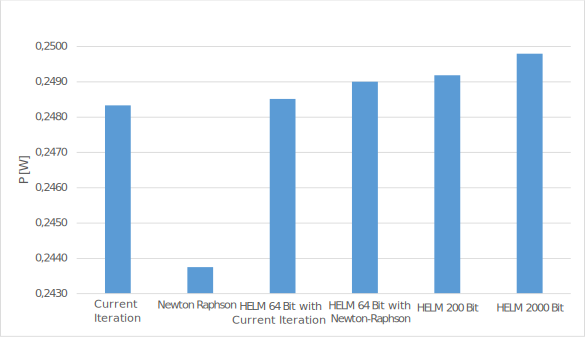
\includegraphics[scale=0.7]{figures/convergence_border}
	\caption{Convergence border for \figinref{convergence_border_net}}
	\label{fig:convergence_border}
\end{figure}

In order to evaluate \emph{HELM} in detail, even for nets close to their border of stability, which can not be calculated with the iterative methods, I decided to implement \emph{HELM} with the possibility of a configurable precise datatype. As the generics in \emph{C\#} did not give me the ability to use a library of precise datatypes together with a package for linear algebra, I decided to implement this part in \emph{C++}. In this language I had templates available, which allowed the combination of \emph{MPIR}\footnote{http://mpir.org/}, a library for multi precision integers and rationals, with a library for sparse linear algebra, like \emph{Eigen}\footnote{http://eigen.tuxfamily.org/}.

\subsection{Linear Algebra}
All the implemented methods have one thing in common: linear algebra. For all these methods it is necessary to solve linear equation systems, although the equation systems differ in their properties. In \emph{HELM} and the \emph{Current Iteration} method the system matrix is the admittance matrix, in \emph{Newton-Raphson} and \emph{FDLF} it is a Jacobian matrix. Both types of matrices are typically sparse, therefore the use of sparse linear algebra improves the performance of the algorithms significantly.

To solve these linear equation systems with a LU-factorization is quite slow for big power nets. One possible  solution is the use of iterative solvers like \emph{BiCGSTAB} \cite{bicgstab}.

Unfortunately, admittance matrices of power nets are sometimes ill-conditioned. Therefore, these iterative solvers may not converge to an accurate result. In order to be able to handle these power nets, it is necessary to reduce the bandwidth of the admittance matrix, for instance through Cuthill-McKee \cite{cuthill}. This method reduces the overhead caused by fill-ins during the LU-factorization. Consequently, the memory usage as well as the total runtime is reduced significantly and it is, again, possible to use the LU-factorization for nets with a six digit number of nodes.

The last important detail of the implementation of the calculation methods is the preconditioning. With this step special properties of the system matrix can be leveraged to improve the condition of the equation system and therefore the iterative solvers are accelerated. Fortunately, the admittance matrix, which is the system matrix in the \emph{Current Iteration} and \emph{HELM}, is approximately diagonal dominant. This makes the application of a diagonal preconditioner very handy because this type of preconditioning is very efficient to calculate. Furthermore, this preconditioning improves the condition of the equation system significantly for admittance matrices.

\subsubsection{Optimizations}
Due to the special circumstances given by \emph{HELM} a few optimizations are possible, however can not be made in general. At the beginning I used \emph{Eigen} for the linear algebra, but with bigger power nets I ran into performance problems with this general purpose library. Consequently, I reimplemented the necessary data structures and algorithms:
\begin{itemize}
	\item Dense vector
	\item Sparse matrix
	\item Multiplication of a sparse matrix with a dense vector
	\item Various operations on dense vectors
	\item \emph{BiCGSTAB}
	\item LU-factorization
	\item Forward and back substitution
\end{itemize}

The specialization on dense vectors is useful in the case of \emph{HELM} as the solutions for the equation system are typically dense. Therefore, there is no need to apply more complex operations on sparse vectors.

However, the system matrix of the linear equation system is the admittance matrix that is sparse for big problems. In fact, the amount of nonzero values in every row is nearly independent of the size of the total matrix. The reason for this lies within the physical structure of a power net, where every node only has a limited number of neighbours, no matter how big the total graph is. Therefore, the density of the admittance matrix decreases with a growing problem size. For small problems this specialization is, in fact, a performance drawback, but for these problems the performance does not matter in any case.

As there must not be a zero-row, a version of a sparse matrix with one array for each row is superior to CRS \cite{sparseMatricesJava} or CCS \cite{sparseMatricesJava}. Through this decision regarding the internal representation of the sparse matrix, during the calculation of the LU-decomposition it is possible to avoid a lot of memory reallocations, which become the most expensive operations if the sparse matrix is represented internally as CRS or CCS. The decision to store the matrices row- and not column-oriented is related to the matrix multiplication and the forward and backward substitution, which benefit from this format in terms of runtime.

The multiplication of a sparse matrix with a dense vector can leverage the special sparse matrix format and the dense vectors. The key point is to iterate only over the nonzero elements over each row in the matrix and select the respective elements of the vector in $\mathcal O(1)$. Additionally, the operation can be parallelized effectively, as all elements in the result vector are independent from each other.

Operations on the dense vectors, like the dot product or adding two vectors, can be parallelized as well. With regards to the performance of the operations, the dense storage of the values is very convenient.

The iterative solver \emph{BiCGSTAB} benefits from the already optimized matrix and vector operations. Additionally, it is possible to avoid a few memory allocations and move operations through implementing all these operations in-place.

The calculation of a LU-factorization and the forward and back subsitution can not benefit from multiple cores well, at least for small datatypes like a double, where the floating point operations are not that expensive. For bigger datatypes with more expensive operations there is also a small speedup possible.

Additionally, I had to concentrate on numerical stability. For this purpose, I sorted all values in ascending order before I summed them up. This special modification has a negative impact on the performance, but it improves the convergence behaviour of \emph{HELM}.

\section{Link to PSS SINCAL}
\label{sec:link_sincal}
The tool developed during this thesis has a parser for the file format of \emph{PSS SINCAL}. This parser allows to read a power net from the file and write back the calculated node voltages.

The basic structure of a power net in \emph{PSS SINCAL} is as follows:
\begin{itemize}
	\item {\textlangle}name{\textrangle}.sin
	\item {\textlangle}name{\textrangle\_}files
	\begin{itemize}
		\item database.001.dia
		\item database.ini
		\item database.mdb
	\end{itemize}
\end{itemize}

The main information about the electrical characteristics of the power net are stored in a database, for instance a \emph{MS Access} database. It is also possible to use \emph{Oracle Database} or \emph{Microsoft SQL Server}. However, during this thesis only nets with a \emph{MS Access} database were used. Therefore, I implemented only a parser for this configuration.

Fortunately, this database is documented very well online\footnote{\url{http://sincal.s3.amazonaws.com/doc/Misc/SINCAL_Datenbankinterface.pdf}; accessed on 14.03.2015} and by the documents delivered together with the application.

The most important relations in this database are:
\begin{itemize}
	\item Terminal: contains information about the connection of the net elements with the nodes
	\item VoltageLevel: mostly used for the frequency of the power net
	\item Element: contains all net elements
	\item Node: contains all nodes with their ID, name, voltage level, ... etc.
	\item TwoWindingTransformer, ThreeWindingTransformer, Line, SynchronousMachine, Load, Infeeder: contain the corresponding net elements
	\item LFNodeResult: contains the node results of the load-flow calculation
\end{itemize}

Of course, \emph{PSS SINCAL} supports a lot more net elements and ways to describe them than the tool developed during this thesis supports. Therefore, for more sophisticated or exotic selections in the database the tool will fail to parse the power net. Especially unsymmetric power nets and short circuit calculations are not supported by this tool. Consequently, the tool neglects the values related to these calculations.

For more detailed information about the database I would like to refer to the official documentation, or the implementation of the parser in the subsystem \emph{SincalConnector}. This part of the software also has a few unit tests, which may be used as documentation too.